% \documentclass[12pt]{ociamthesis}  % default square logo
\documentclass[12pt]{article}  % default square logo

\usepackage[margin=2.8cm]{geometry}
\usepackage{setspace}
\usepackage{mathptmx} % Times font
\usepackage{mathrsfs} % mathrsfs font
\usepackage[utf8]{inputenc}
\usepackage{graphicx}
\usepackage{framed}
\usepackage{hyperref}
\usepackage{amssymb} % empty set

% code listing
\usepackage{listings}
\usepackage{xcolor}

% packages for drawing
\usepackage{tikz}
\usetikzlibrary{graphs}     % create graphs
\usetikzlibrary{arrows}

%% set code styles

\definecolor{dkgreen}{rgb}{0,0.6,0}
\definecolor{gray}{rgb}{0.5,0.5,0.5}
\definecolor{mauve}{rgb}{0.58,0,0.82}

\lstset{
  frame=tb,
  language=scala,
  aboveskip=3mm,
  belowskip=3mm,
  showstringspaces=false,
  columns=flexible,
  basicstyle={\small\ttfamily},
  numbers=none,
  numberstyle=\tiny\color{gray},
  keywordstyle=\color{blue},
  commentstyle=\color{dkgreen},
  stringstyle=\color{mauve},
  breaklines=true,
  breakatwhitespace=true,
  tabsize=3,
}

% definitions, theorems

\newtheorem{definition}{Definition}


\onehalfspacing

%end the preamble and start the document
\begin{document}

\begin{titlepage}

  \begin{center}

    %% \vspace{20cm}
    \vspace*{3\baselineskip}
    % Title
    {\Large Dependency Resolution Through SAT Solvers \\[0.4cm] }
    {\bfseries Experiments on Maven and Ivy Ecosystems\\[1.5cm] }

    % Author and supervisor
    \noindent
    Fengyun \textsc{Liu} \\[0.3cm]

    \noindent
    {School of Computer and Communication Sciences \\[2cm]}

    \begin{framed}
    Semester Project \\
    Professor: Martin Odersky \\
    Supervisor: Nada Amin \\
    %% Programming Methods Laboratory \\
    Report accepted on \today
    \end{framed}

    \noindent
    Lausanne, academic year 2014 - 2015 \\[1cm]

    % Upper part of the page. The '~' is needed because \\
    % only works if a paragraph has started.
    
\includegraphics[width=0.8\textwidth]{img/epfl}~\\[1cm]

    %\vfill

    % Bottom of the page
    %% {\large \today}

  \end{center}

\end{titlepage}

%% \include{content/dedication}        % include a dedication.tex file
%% \include{content/acknowlegements}   % include an acknowledgements.tex file
\begin{abstract}
  This report introduces a new algorithm to resolve software package dependency for Ivy and Maven ecosystems by using off-the-shelf SAT solvers. This algorithm avoids the common problem in Maven and Ivy, which rely on conflict resolution even when there're no conflicts, which produces confusing results to end users sometimes.

Besides, the new algorithm can elegantly handle the case of missing dependencies or conflicts by showing the error as a tree, which makes it clear to end users how the root dependencies lead to the error transitively.

%  The algorithm is practically fast enough, which makes it an ideal candidate for improving existing dependency management tools.

This report also discusses pragmatics that are related to software package dependency management in general. I argue for the separation of project specification and artifact specification, and a restriction on the features of artifact specification. These reflections might be helpful for future ecosystem designers.

\end{abstract}
          % include the abstract

\pagenumbering{Roman}
\tableofcontents            % generate and include a table of contents
% \listoffigures              % generate and include a list of figures

\pagenumbering{arabic}
%now include the files of latex for each of the chapters etc
\section{Introduction}

Software packages are widely used in software development to improve productivity. However, usage of software packages can be difficult, which is widely known as the \emph{dependency hell}.

This section briefly explains why usage of software packages is difficult and the motivation for experimenting a new algorithm.

\subsection{Why usage of packages is difficult}
Usage of software packages is complicated by \emph{package versioning}, \emph{transitive dependency} and \emph{complex dependency constraints}.

Software packages evolve over time, some supported features might no longer be supported afterwards, some interface might be changed or deprecated later. Software packages are usually versioned by some \emph{versionning scheme} to clearly mark the changes in each version. Users of a package should know the exact version that's been used to make sure it supports all the required features and the documentation conforms to the specific version.

Software package dependency is transitive. If a package $x$ depends on a package $y$, and $y$ depends on a package $z$, then $x$ depends on $z$. Though developers specify the dependencies as a flat list, it usually expands to a complex directed graph.

Dependency specification requires the support of complex constraints, like \emph{fuzzy version constraints}, \emph{excludes in transitive dependency}, \emph{intransitive dependency}, etc. For example, a project may need to specify fuzzy version constraints, such as $(, 1.0.0]$, $[1.5.2, 1.6.0)$, etc. Sometimes there's the need to exclude a specific package from all later transitive dependencies or to mark a dependency as intransitive.

The complexity in software packages may lead to two problems -- one is \emph{conflict}, the other is \emph{missing dependency}. Usually, only one version of a package can be used in the same project. If a project transitively depends on two different versions of the same package, then there's a \emph{conflict}. On the other hand, if a project depends on a package that can't be found, then there's a \emph{missing dependency}.

The complexity with the usage of packages necessitates tools to automatically check whether a dependency specification can be satisfied or not. More concretely, a dependency manager has to check that for a given dependency specification (1) whether there exists conflicts or missing dependencies; (2) if there's no error, generate an optimal set of packages so that the dependency constraints of the specification and of each package in the solution set are satisfied.


\subsection{Motivation of the project}

In the Java world, Maven\footnote{\url{https://maven.apache.org}} and Ivy\footnote{\url{http://ant.apache.org/ivy/}} are the two most widely used dependency management tools.

The common problem with Ivy and Maven is that they resort to conflict resolution unnecessarily even when the specification is satisfiable with no conflicts. This is better illustrated with Figure \ref{fig:introuction:underconstraint}, where the rectangles represent versioned packages, and the rounded rectangles represent dependency constraints.  As we can see in the graph, the project depends on the package A and B directly, and they in turn depend on the package C.

\begin{figure}[ht]
  \center
  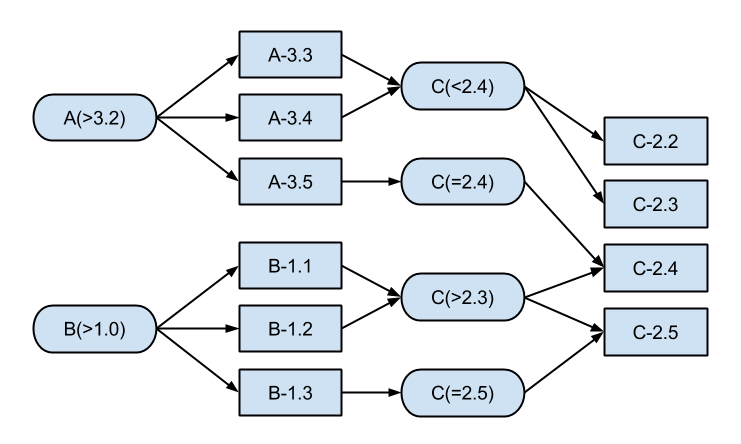
\includegraphics[width=14cm]{img/introduction/underconstraint.png}
  \caption[An example dependency graph]{An example dependency graph \label{fig:introuction:underconstraint}}
\end{figure}

It's obvious that the dependency graph in Figure \ref{fig:introuction:underconstraint} has a solution set $\{(A, 3.5), (B, 1.2), (C, 2.4)\}$. However, both Maven and Ivy would think there's a conflict on the package $C$, and the conflict manager would be called to resolve the conflict. Depending on the setting of the conflict manager, usually $(C, 2.5)$ will be chosen, which is incorrect! This behavior is documented on Ivy official web site\footnote{\url{http://ant.apache.org/ivy/history/latest-milestone/principle.html}}:

\begin{quote}
  When the dependency module has been found, its ivy file is downloaded to the ivy cache. Then ivy checks if the dependency module has dependencies, in which case it recursively traverses the graph of dependencies.

  All over this traversal, conflict management is done to prevent access to a module as soon as possible.
\end{quote}

The popular build tool Gradle\footnote{\url{https://gradle.org}} has the similar problem, as documented in section \emph{50.7. How dependency resolution works} on their official site\footnote{\url{https://docs.gradle.org/current/userguide/dependency_management.html}}.

In Scala, Sbt\footnote{\url{http://www.scala-sbt.org}} depends on Ivy to resolve dependencies, so it inherits the problem. It produces confusing resolution results to users sometimes. The motivation for this project is to experiment with a new algorithm based on SAT solvers to avoid this problem. If proved feasible, sbt can drop the dependency on Ivy and use the new algorithm in the future to avoid the problem.

\subsection{Contributions of the project}

This project has two major contributions. First, the successful application of SAT solvers to dependency resolution both for the Maven and the Ivy ecosystem. There has already been many applications of SAT solvers in dependency management\cite{mancinelli2006managing, berre2009dependency, vouillon2013software}, but implementation of the method for the Maven and Ivy ecosystem in the context of software development is a new attempt. This project demonstrates that this approach is feasible.

Second, based on argumentative reasoning, this report proposes the separation of project specification and artifact specification, and a restriction on the features of artifact specification. These reflections might be helpful for future ecosystem designers.

\section{Dependency Management through SAT Solvers}

In this section, I'll describe in detail how the new algorithm works. The resolution algorithm consists of two independent algorithms:

\begin{enumerate}
\item An algorithm to construct a local repository based on the transitivity of dependency.
\item An algorithm to use an SAT solver to find an optimal solution on the local repository.
\end{enumerate}

The first algorithm, which I call the \emph{closure construction algorithm}, recursively constructs a repository whose packages are the transitive closure of the initial constraints. In the process of constructing the local repository, it has to handle particular features of Maven and Ivy, such as \emph{fuzzy constraints}, \emph{excludes}, \emph{intransitive dependencies}, \emph{forces}, \emph{scopes} or \emph{configurations}. We need two versions of the algorithm here, one for Maven and one for Ivy.

The second algorithm, which I call the \emph{encoding algorithm}, encodes the local repository to the format of a specific SAT solver, and decodes the result to a user-friendly format. We only need one version of this algorithm.


\subsection{Formalism}

Formalization of the problem based on set semantics is the first step to solve the problem via SAT solvers. The formalism used here is based on the work of Mancinelli et al.\cite{mancinelli2006managing}.

There is a big disparity between the concepts in the Maven ecosystem and the Ivy ecosystem. For example, a package in Maven is very different from a package in Ivy. In Maven, a package is the same as an artifact, but in Ivy a package may define several artifacts. The difference can be abstracted away for the purpose of dependency management based on following two concepts.

\begin{definition}[Library]
  A library is a unique entity which can be versioned.  The versioning of a library should be a total-order. In the Java world, a library is usually identified by the pair $(group, name)$.
\end{definition}

\begin{definition}[Package]
  A package is a versioned library. Two packages of the same library but of different versions conflict.  A package can be denoted as a pair $(l, v)$.
\end{definition}

% \subsubsection{Fuzzy Constraints}

\noindent
\textbf{Fuzzy Constraints}. It's possible to specify fuzzy constraints both in Maven and Ivy. For example, a package $p$ may dependent on $x(\geq 2.3)$. To encode the fuzzy constraints, we can expand $x(\geq 2.3)$ to a set of  concrete packages, such as $\{x_1, x_2, x_3, ...\}$.

Following the approach above, it's possible to encode the direct dependency constraints of any package as a set of sets of packages. This insight enables us to formalize the concept \emph{repository}\cite{mancinelli2006managing}.

\begin{definition}[Repository]
  A repository is a tuple $R = (P, D, C)$ where $P$ is a set of packages, $D : P \rightarrow \mathscr{P p 1}(\mathscr{P p 1}(P))$ is the dependency function\footnote{$\mathscr{P p 1}(X)$ represents the set of subsets of X.}, and $C \subset P \times P$ is the conflict relation. The repository must satisfy the following conditions:

  \begin{itemize}
  \item The relation $C$ is symmetric, i.e., $(\pi_1, \pi_2) \in C$ if and only if $(\pi_2, \pi_1) \in C$ for all $\pi_1, \pi_2 \in C$.
  \item Two packages with the same unit but different versions conflict, i.e., if $\pi_1 = (l, v_1)$ and $\pi_2 = (l, v_2)$ with $v_1 \neq v_2$, then $(\pi_1, \pi_2) \in C$.
  \end{itemize}
\end{definition}

In a repository $R = (P, D, C)$, the dependencies of each package $p$ are given by $D(p) = \{d_1, ..., d_k\}$, which is a set of sets of packages. It means if $p$ is to be used, then all its $k$ dependency requirements must be satisfied. For the constraint $d_i$ to be satisfied, at least one of the packages in $d_i$ must be used as well.

For example, if $D(p) = \{\{a_1, ..., a_k\}, \{c_1, ..., c_j\}\}$, then in order to use $p$, at least one package in $\{a_1, ..., a_k\}$ and one in $\{c_1, ..., c_j\}$ must be used.

Now we can formalize the concept \emph{resolution}.

\begin{definition}[Resolution]
  A resolution for the initial package $\pi$ with regard to a repository $R = (P, D, C)$ is a subset $I$ of $P$. The resolution $I$ must satisfy following conditions:

  \begin{itemize}
  \item \emph{Inclusion}: The initial package is in the resolution. Formally, $\pi \in I$.
  \item \emph{Abundance}: Every package has what it needs. Formally, for every $\pi \in I$, and for every dependency $d \in D(\pi)$ we have $I \cap d \neq \emptyset$.
  \item \emph{Peace}: No two packages conflict. Formally, $(I \times I) \cap C = \emptyset$.
  \end{itemize}
\end{definition}

Note that a resolution may not always exist. There could be conflicts or missing dependencies. In the following, I use \emph{root package} as a synonym of \emph{initial package}, and \emph{root dependencies} means the dependencies of the root package.

\subsection{Closure Construction Algorithm}

The closure construction algorithm is basically a depth-first-search(DFS) algorithm on the \emph{flattened dependency graph} of the closure repository of the root package, which is defined as follows.

\begin{definition}[Flattened Dependency Graph]
  The flattened dependency graph $G = (N, E)$ for a repository $R = (P, D, C)$ is a directed graph, where the nodes are the packages, and the arcs are the dependencies between packages. Formally, $N = P$, and $E = \{ (p, q) | \exists d_i \in D(p) \land q \in d_i\}$.
\end{definition}

Note that there could be cycles in the graph. Following example demonstrates how cycles could arise in practice.

\begin{verbatim}
(x, 2.3) depends on y(>=1.3)
(y, 1.4) depends on x(>=2.1)
\end{verbatim}

It's obvious that in the example above, there is an arc from $(x, 2.3)$ to $(y, 1.4)$, because $(y, 1.4) \in \{(y, v) | v \geq 1.3 \}$. For similar reasons, there is an arc from $(y, 1.4)$ to $(x, 2.3)$. Thus, in this case there is a cycle in the flattened dependency graph. The existence of cycles in the graph implies that the algorithm should keep track of visited nodes in order to avoid infinite loops.

The algorithm is implemented as a recursive function in Scala, which has following signature:
\begin{lstlisting}[language=Scala]
  // Maven
  def resolve(pom: MDescriptor, scope: Scope,
               excludes: Iterable[LibT], path: Set[PackageT]): Unit
  // Ivy
  def resolve(ivy: IDescriptor, confs: Set[String],
               excludes: Seq[IExclude], path: Set[PackageT]): Unit
\end{lstlisting}

The algorithm starts from the root package, and advances following the depth-first-search approach on the flattened dependency graph of the closure repository. In the visiting process, the algorithm updates two mutable data structures $packagesMap$ and $librariesMap$:

\begin{lstlisting}[language=Scala]
  // Maven
  type DependenciesT = Set[(MDependency, Set[MPackage])]

  val packagesMap = new TrieMap[MPackage, DependenciesT]
  val librariesMap = new TrieMap[ILib, Set[MPackage]]

  // Ivy
  type DependenciesT = Set[(IDependency, Set[IPackage])]

  case class PackageInfo(dependencies: DependenciesT, descriptor: IDescriptor,
                          activeConfs: Set[String], activeArtifacts: Set[String])

  val packagesMap = new TrieMap[IPackage, PackageInfo]
  val librariesMap = new TrieMap[ILib, Set[IPackage]]
\end{lstlisting}

Compared to the repository triple $R = (P, D, C)$, the structure $packagesMap$ is the representation of the dependency function $D$, and as $P$ is the domain of $D$, thus is represented by the keys of $packagesMap$. The structure $librariesMap$ is a representation of conflicts $C$. Additional information is maintained in $packagesMap$ for more detailed resolution report.

In the following, I'm going to introduce in detail how the particular features of Maven or Ivy are handled by the \emph{closure construction algorithm}.

\subsubsection{Fuzzy Constraints}

Fuzzy constraints are expanded to individual packages as mentioned before. To handle a fuzzy constraint $L(pred)$, the algorithm first retrieves a list of all versions of the library $L$, then select valid versions by the constraint predicate $pred$.

In Scala, the relevant code snippet is as follows:

\begin{lstlisting}[language=Scala]
  // Maven
  metaResolver(dep.lib).map(dep.filterVersions)

  // Ivy
  versionsResolver(dep.lib).map(dep.filterVersions)
\end{lstlisting}

\subsubsection{Intransitive Constraints}

Ivy supports intransitive dependencies. To support this feature, only advance the depth-first-search if current dependency is transitive. In Scala, we only need to add a conditional check before the recursive call:

\begin{lstlisting}[language=Scala]
  if (dep.transitive)
      resolve(descriptor, depConfs, newExcludes, path + ivy.pkg)
\end{lstlisting}

\subsubsection{Scopes or Configurations}

Maven supports \emph{scopes}, Ivy supports a similar but more flexible concept \emph{configuration}. To support this feature, they are added to the signature of the recursive function:

\begin{lstlisting}[language=Scala]
  // Maven
  def resolve(pom: MDescriptor, scope: Scope, ...): Unit = {
    val deps = pom.filterDependencies(scope, excludes)
    deps.foreach { dep =>
      val newScope = COMPILE
      // ...
    }
  }

  // Ivy
  def resolve(ivy: IDescriptor, confs: Set[String], ...): Unit = {
    val deps = ivy.filterDependencies(confs, excludes)
    deps.foreach { dep =>
      val newConfs = ivy.filterDepConfigurations(confs, dep)
      // ...
    }
  }
\end{lstlisting}

The first line in the body of the function filters the effective dependencies according to the semantics of scope and configurations respectively.

For Maven, the new scope is always \emph{compile}, because Maven scopes are fixed, and it doesn't make sense for one package to depend on scopes other than \emph{compile} of another package.

For Ivy, the new configurations are calculated for each dependency according to the dependency mapping of configurations defined in the descriptor.

\subsubsection{Excludes}

\label{sat:excludes}

Both Maven and Ivy support excludes in dependency. This feature complicates the \emph{closure construction algorithm}. Ideally, each package in the \emph{flatten dependency graph} is visited once. However, the effective scope of excludes is along the transitive chain, it's possible that for a dependency $d$ of a package $\pi$, it's excluded in one chain, but included in another chain. This is illustrated by following example:

\begin{verbatim}
p   depends on(exclude=t)   h(deps={t(>2.1)})
q   depends on   h(deps={t(>2.1)})
\end{verbatim}

In the example above, the dependency path from $p$ to $h$ excludes the library $t$, while the dependency path from $q$ to $h$ includes $t$. This implies we should allow each package to be visited multiple times along different paths, and the dependencies of different paths should be added together by the set union operation. As the combination of paths in a graph could be exponential, the cost in path traversal is potentially exponential. That's one of the reason why I think we should restrict features in artifact specification. I'll discuss more about the topic in section \ref{pragmatics}.

The parameter \emph{path} in the signature represents the visited path. The parameter \emph{excludes} represents the effective excludes.

\begin{lstlisting}[language=Scala]
  // Maven
  def resolve(pom: MDescriptor, scope: Scope,
               excludes: Iterable[LibT], path: Set[PackageT]): Unit
  // Ivy
  def resolve(ivy: IDescriptor, confs: Set[String],
               excludes: Seq[IExclude], path: Set[PackageT]): Unit
\end{lstlisting}

Inside the function body, the excludes are used to filter effective dependencies. Both the \emph{exludes} and \emph{path} are accumulated along the visited path, but different paths don't interfere with each other.

\subsubsection{Overrides}

Ivy supports specifying an override mediation rule, overriding the revision requested for a transitive dependency. This feature can be useful when a direct dependency is bringing a transitive dependency for which the programmers want to change the revision, without actually declaring a dependency on it (because the module doesn't actually depend on it).

Current implementation doesn't support this feature, but technically it's similar to the support of \emph{excludes}, which is also effective and accumulative along the transitive dependency chain.

When interpreting a dependency constraint $L(pred)$, the algorithm should first check if the library $L$ is covered in the \emph{overrides} set. If it's, then the version constraint $pred$ should be replaced by the version constraint specified in the override rules.

In case where there are two override rules on the same library, the override rule closer to the root package has higher precedence\footnote{The Ivy official web site doesn't document how to handle such cases. This is just a reasonable proposition.}.

\subsubsection{Force}

Ivy supports a boolean flag \emph{force} on a dependency constraint, which says that this dependency
should be forced to the specified revision. The effective scope of \emph{force} is global\footnote{Ivy documentation is obscure about this point, but that seems to be the only reasonable interpretation. \\\url{http://ant.apache.org/ivy/history/latest-milestone/ivyfile/dependency.html}} -- instead of being along the transitive dependency chain -- it means if a specific version of a library $L$ is forced, it has to override all dependencies on $L$ for every package in the repository.

The global effective scope of \emph{force} implies we should do post-processing on the dependencies of each package in order to make \emph{force} effective. If there are multiple \emph{forces} on the same library, then it's up to the solver to select one from them -- usually the latest version is chosen\footnote{The Ivy official web site doesn't say anything about the scenario, it's just a reasonable proposition.}.

This feature has not been implemented yet. But given the semantics above, it's not hard to implement this feature by keeping track of all forces during graph traversal, and then do post-update on dependencies of forced libraries for each package.

\subsection{Encoding Algorithm}

Once the local repository has been constructed, the \emph{encoding algorithm} can encode the repository into a SAT problem and call a SAT solver to find a resolution. The encoding algorithm depends on an abstract representation of repository, which has following signature:

\begin{lstlisting}[language=Scala]
  abstract class Repository { outer =>
    type LibT   <: Lib
    type PackageT    <: Package { type LibT = outer.LibT }
    type DependencyT <: Dependency { type LibT = outer.LibT }

    /** Returns the root package of the repository */
    def root: PackageT

    /** Returns the packages that p depends on directly */
    def apply(p: PackageT): Iterable[(DependencyT, Iterable[PackageT])]

    /** Returns all packages in the repository, except the root */
    def packages: Iterable[PackageT]

    /** Returns all primitive conflicts in the repository */
    def conflicts: Map[LibT, Set[PackageT]]
  }
\end{lstlisting}

This abstract interface enables us to use the same encoding algorithm for both Maven and Ivy. In the following I'll explain in detail how to encode the repository into a SAT problem. I'll keep the introduction abstract, so that it's possible to switch to other SAT solvers following the tricks introduced here. For readers interested in the details of encoding the problem in SAT4J, please refer to our code base on Github\footnote{\url{https://github.com/liufengyun/bacala/blob/master/src/main/scala/bacala/alg/SatSolver.scala}}.

The encoding tricks are based on the work of Berre et al. \cite{berre2009dependency}. The implementation is based on SAT4J Pseudo\footnote{\url{http://www.sat4j.org}} version $2.3.4$.

\subsubsection{Encode Dependency}

Remember that in our formalism of a repository $R = (P, D, C)$, the dependency of a package $p$ is like $D(p) = \{\{a_1, ..., a_k\}, \{c_1, ..., c_j\}\}$. It means in order to use $p$, at least one package in $\{a_1, ..., a_k\}$ and one in $\{c_1, ..., c_j\}$ must be used. If we take each package as a proposition variable, this naturally translates to following logical formula:

\[
p \rightarrow ((a_1 \vee ... \vee a_k) \wedge (c_1 \vee ... \vee c_j))
\]

Generally, for a package $p$ with $D(p) = \{ d_1, d_2, ..., d_n\}$ and $d_i = \{ q_{i, j} | i \leq j \leq m_i \}$, it can be encoded as following logical formula:

\[
p \rightarrow \bigwedge_{1 \leq i \leq n} \bigvee_{1 \leq j \leq m_i} q_{i,j}
\]

Some SAT solvers require the input in \emph{conjunctive normal form}, which can be derived as follows:

\[
p \rightarrow \bigwedge_{1 \leq i \leq n} \bigvee_{1 \leq j \leq m_i} q_{i,j}
\quad \quad \equiv \quad \quad
\bigwedge_{1 \leq i \leq n} p \rightarrow \bigvee_{1 \leq j \leq m_i} q_{i,j}
\quad \quad \equiv \quad \quad
\bigwedge_{1 \leq i \leq n} (\neg p \vee \bigvee_{1 \leq j \leq m_i} q_{i,j})
\]

If the package $p$ is the root package, it's always required. Thus the dependency of the root package can be encoded by dropping the implication:

\[
\bigwedge_{1 \leq i \leq n} \bigvee_{1 \leq j \leq m_i} q_{i,j}
\]

\subsubsection{Encode Conflicts}

For given a repository $R = (P, D, C)$, the conflicts $C$ is a set of pairs like $(p, q)$. A natural approach is to encode the conflict pair $(p, q)$ as $\neg p \vee \neg q$. Then all conflicts in the repository can be encoded as following formula:

\[
\bigwedge_{(p, q) \in C} \neg p \vee \neg q
\]

A slightly different encoding is based on the fact that all package conflicts in software development are due to version conflicts on the same library. Suppose the function $CL(L)$ returns all versions of the library $L$ in the repository, then it's possible to encode the conflict on library $L$ as a cardinality constraint\footnote{Cardinality constraint is supported by all major SAT solvers}:

\[
(\sum_{p \in CL(L)} p) \leq 1
\]

In the implementation, the second approach is taken. Unlike the comment in \cite{berre2009dependency}, which claims the second approach is superior for error reporting, we observed no such advantage in our implementation. We take the second approach mainly because it makes logical translation simpler.

\subsubsection{Choose the Optimal Solution}

There could be multiple resolutions for a given repository. In that case, an optimal solution should be chosen. In the context of software package dependency management, new versions of a library are preferred over old versions of a library, so the solver should favor the solution which contains the newest versions of libraries.

SAT4J supports setting a \emph{pseudo-boolean function} to minimize for resolution. The objective function has following form:

\[
\sum_{p \in P} w_p p
\]

So the problem becomes \emph{how to define the weight for each package $p$ in the repository}. The approach we take is rank-based weight. For each library, we rank all versions of the library in the repository, newer versions get lower ranks. Then we use the rank of a package for its weight in the objective function.

This approach works well in our experiment, and it's better than approaches that depend on version numbers, as the latter are prone to version skew, where the library has large version numbers will be dominating in the objective function. The rank-based approach can be seen as having performed a normalization step on the version numbers.

\subsubsection{Report Friendly Error Message}

In case there is no solution for a given repository, the algorithm should report friendly error messages to end users. There are two problems related to user-friendliness.

First, as each library has several candidate versions in the repository, there are many combinations of packages where missing dependencies or conflicts can happen. A user friendly approach is to choose the minimal combination of packages where this is no solution.

Second, as conflicts or missing dependencies can happen very deep in the graph, just reporting these errors will confuse end users, as these packages are not directly required by the root package. A friendly error report should relate the missing dependencies or conflicts to the root dependencies.

From the logical point view, the first problem is equivalent to find the minimal subset $T$ of the total formulas $S$ that cannot be satisfied altogether. This subset of formulas is also called MUS(\emph{minimal unsatisfiable subformula}). Formally, $T$ is MUS of $S$ if and only if $T \subseteq S$, $T \vDash \perp$ and $\nexists R \subset T \wedge R \vDash \perp$.

An elegant algorithm to compute MUS is QuickXplain\cite{junker2004quickxplain}. The algorithm has the merit that it doesn't require any change to the SAT solver. QuickXplain works by translate the constraints $S = \{ s_1, ..., s_n\}$ into $S'$ by adding a new selector variable $sel_i$ to each constraint in $S: S' = \{ sel_1 \vee s_1, ..., sel_n \vee s_n\}$. Then the problem is transformed into a pseudo-boolean problem to minimize the objective function $\sum_{1 \leq i \leq n} sel_i$ under the constraint $S' \bigwedge_{1 \leq i \leq n} \neg sel_i$, which can be readily solved by existent SAT solvers.

To deal with the second requirement, we need to relate each translated logical formula to the original dependency in the repository. When the SAT solver produces MUS, we are sure that the dependencies that correspond to the formulas must form paths from the root package to the place where missing dependencies or conflicts happen. Otherwise, it's possible to show the the set of unsatisfiable subformula is not minimal, which is a contradiction.

Based on this observation, we are able to display the missing dependencies or conflicts as a tree from the root package to the level where the error happens, which makes it clear to end users how the root dependencies lead to the error transitively.

\subsection{Performance}

For the POM and Ivy files we tested, the SAT resolver never takes more than one second. The largest POM file we tested has 46 packages in the solution set, and it took 0.17 second on SAT solver, 68.4 seconds in downloading POM files. With local file system caching of POM files, the cost of network IO drops quickly after the first run on the project.

% When all the POM and Ivy files are cached locally, the new algorithm is about 30 times faster than Maven and Ivy.

\section{Pragmatics of Dependency Management}

\label{pragmatics}

To elegantly solve the software dependency problem and avoid the dependency hell, it requires not only good resolution algorithms, but also good practices. For example, \emph{semantic versioning}\footnote{\url{http://semver.org}} is widely recognized to be a good practice in package versioning.

In this section, I'll argue for (1) the separation of project specification and artifact specification, and (2) a restriction on the features of artifact specification. I hope this analysis will be useful for future ecosystem designers.

\subsection{Separation of Project Specification and Artifact Specification}

By \emph{project specification} I mean the specification of package dependencies in development, which is usually checked into the version control system along with the project code\footnote{It's possible to distinguish two different usage of project specification -- one for application, and one for library. They are the same in most places, but may diverge on some features. However, I'm not going to pursue the nuances between them here.}. By \emph{artifact specification} I mean the specification that locates on repository server which describes the name, version and dependencies of a reusable artifact.

I propose that it's good to separate project specification and artifact specification, and use different specification languages for them.

The most important reason is that they target different audience. Project specifications are read and written by programmers, while artifact specifications are usually generated and read by programs. Project specifications change as the projects evolve, while artifact specifications stay the same once created. DSL is suitable for project specifications, while XML is suitable for artifact specifications. In this regard, SBT and Gradle are on the right track.

Besides, project specification and artifact specification need different features. This is discussed in detail in next section.

\subsection{Evaluation of Features}

In this section, I present an evaluation about which features are appropriate in which context. The result is summarized in Table\ref{table:prag:features}. In the following, I'm going to justify each row of the table one by one.

\begin{table}
  \center
  \begin{tabular}{|l|c|c|}
    \hline
    Features              & Project Specification & Artifact Specification \\
    \hline
    Language              &   DSL                 & XML \\
    Fuzzy Constraints     &   Yes                 & Yes \\
%    Fixed Constraint      &   Yes                 & No \\
    Resolvers             &   Yes                 & No \\
    %% Force                 &   Yes                 & No \\
    Intransitive          &   Yes                 & No \\
    %% Substitution          &   Yes                 & No \\
    Excludes              &   Yes                 & No \\
    Overrides             &   Yes                 & No \\
    Configurations        &   Yes                 & No \\
    Multiple Artifacts    &   Yes                 & No \\
    Build Tasks           &   Yes                 & No \\
    \hline
  \end{tabular}
  \caption[Features Comparison]{Features comparison between project specification and artifact specification \label{table:prag:features}}
\end{table}

\textbf{Fuzzy Constraints}. Usage of fuzzy constraints should be encouraged, as it reduces potential version conflicts. Based on \emph{semantic versioning}, fuzzy constraint is a good feature for both project specification and artifact specification. In contrast, while usage of strict constraints(a specific version) in an application project specification can be justified, its usage in artifact specification is discouraged, as it is prone to version conflicts.

\textbf{Resolvers}. A project specification may contain information about resolvers(remote repositories), but it doesn't make sense to put this information in the artifact specification, as an artifact might be placed in a lot of places and the information may change over time. Ivy moved resolvers to setting files, which is an improvement over Maven.

% \textbf{Force}. Force tells the dependency manager to use a specific version of a library even if there is conflict. It's reasonable to use this feature sometimes at the risk of the programmer in development. Usage of \emph{force} should be forbidden in artifact specification, as it imposes an unconditional decision on all projects where the package is used, which is an aggression on the freedom of projects.

\textbf{Intransitive}. Intransitive dependency doesn't make sense in artifact specification because marking a dependency as intransitive depends on some assumptions about the environment. These assumptions may not necessarily hold in all usages of the artifact. In the context of project development, it's relatively safe to make assumptions and the feature can be used at the risk of the programmer.

\textbf{Excludes}. Excludes tells the dependency manager to exclude dependencies on some libraries. For similar reasons as \emph{intransitive}, the usage of \emph{excludes} is resolution-context-sensitive, while artifact specification should be as resolution-context-free as possible.

Another reason against the usage of excludes in artifact specification is about performance. As it's mentioned in section \ref{sat:excludes}, the effective scope of excludes is along the transitive path. As the combination of paths in the graph is exponential, which may lead to exponential blow up even in simple dependency graphs. This line of argument also holds for \emph{overrides}.

\textbf{Overrides}. Overrides tells the dependency manager to use a specific version of a library for all dependencies on the library. Like \emph{excludes}, the usage of \emph{overrides} is resolution-context-sensitive, thus it should not appear in artifact specification, which is assumed to be resolution-context-free. Usage of overrides imposes an unconditional decision on all projects where the package is used, which is an aggression on the freedom of projects.

\textbf{Configurations}. Project specifications may contain several different configuration, such as test, production, etc. However, it doesn't make sense to have several configurations in an artifact specification, as when an artifact is required, it's expected to behave the same in different contexts.

\textbf{Multiple Artifacts}. It makes sense for a library project specification to define multiple artifacts, but it doesn't make sense for an artifact specification to specify more than one artifact, as artifact is the unit of reuse and dependency. Specifying more than one artifact in the specification complicates usage. In this regard, the design of Ivy is terrible.

\textbf{Build Tasks}. It's reasonable to define build tasks in a project specification, but it doesn't make sense to define build task inside an artifact specification, as it is useless.

I think these arguments are enough to support our initial proposition. Upon inspection of real world tools, we find SBT and Gradle are on the right track. Ivy and Maven are inadequate because they don't provide a friendly project specification language for programmers, and also because they provide too many features for artifact specifications, which is problematic.

\section{Conclusion}

Our project has shown that usage of SAT solvers for dependency management is not only theoretically possible, but also practically feasible. This algorithm avoids the common problem in Maven and Ivy -- which rely on conflict resolution even when there is no conflict -- and produces more correct answers. And the algorithm can report the error as a dependency tree when there is missing dependency or conflict, which makes it clear to end users how the root dependencies lead to the error transitively.

% The algorithm is practically fast enough, which makes it an ideal candidate for improving existing dependency management tools.

\subsection{Future Work}

As we've seen, in the new resolution algorithm, the time spent on network IO is dominating, the time spent on SAT solver is insignificant. If the POM or Ivy files are local, the algorithm would be extremely fast.

This implies we can use a central server for dependency resolution. The client sends the dependency specification to the server, the server does dependency resolution and sends the result back to the client. The client only needs to download artifacts from repositories. The rationale behind this is that when it's expensive to move data to computation, it's reasonable to move computation to data.

In the process of resolving dependency, the server downloads POM or Ivy files from repositories and cache them locally. The more POM and Ivy files the server caches, the faster the server will be.

For companies which have private repositories, they can set up private servers for dependency resolution.

\subsection{Acknowledgments}

I thank Nada Amin for her supervision of this semester project. Her guidance saved me a lot of time in searching relevant literature and enabled me to attack on the problem directly without any zigzag. I thank Josh Suereth for his valuable feedback on the implementation of the project.


%now enable appendix numbering format and include any appendices
%% \appendix
%% \include{content/appendix1}

%next line adds the Bibliography to the contents page
\addcontentsline{toc}{section}{Bibliography}
%uncomment next line to change bibliography name to references
%\renewcommand{\bibname}{References}
\bibliography{refs}        %use a bibtex bibliography file refs.bib
\bibliographystyle{plain}  %use the plain bibliography style

\end{document}
